\question Albert keeps all of his top secret information in a binary tree. To protect the information,
Albert turns some of the nodes in his trees into \lstinline$Eert$ nodes. \lstinline$Eert$ nodes, which have
\lstinline$Tree$ as their base class, are like normal \lstinline$Tree$ nodes, except they swap their left
and right branches. (Albert settles for nothing less than the most advanced encryption techniques
known to man.)

\begin{parts}
\part On the next page, complete the \lstinline$__init__$ method for the \lstinline$Eert$. Make sure to use
inheritance as much as possible. The \lstinline$Eert$ class should work as follows:

\begin{lstlisting}
>>> e = Eert('61A account info',
... Tree('Username: cs61a-te'),
... Tree('Password: imsocool'))
>>> e.entry  # unchanged
'61A account info'
>>> e.left.entry  # swapped with right
'Password: imsocool'
>>> e.right.entry  # swapped with left
'Username: cs61a-te'
\end{lstlisting}

\part On the next page, complete the definitions of the \lstinline$decrypt$ methods for both the
\lstinline$Tree$ and \lstinline$Eert$ classes. When the \lstinline$decrypt$ method is invoked on a binary tree
containing \lstinline$Tree$ and \lstinline$Eert$ nodes, it returns a copy of the binary tree, but with all
\lstinline$Eert$ nodes replaced with \lstinline$Tree$ nodes. During this replacement, you should also swap
the \lstinline$left$ and the \lstinline$right$ back to their proper positions! Here is a graphical
representation of the process:

\begin{minipage}{0.5\linewidth}
Original:

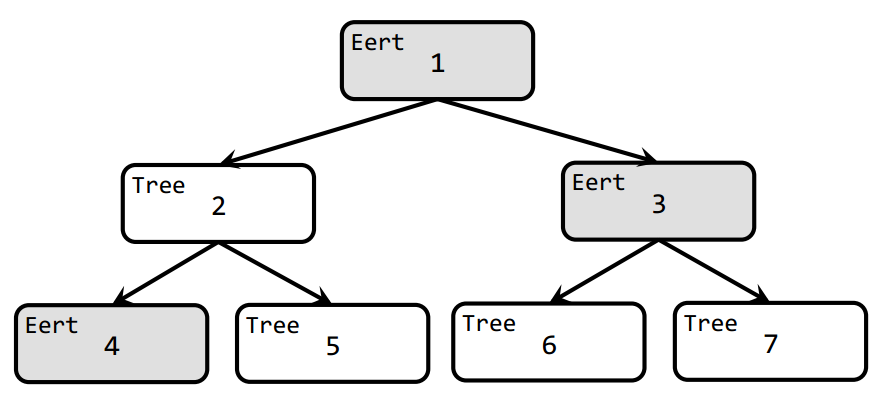
\includegraphics[width=\linewidth]{original.png}
\end{minipage}
\begin{minipage}{0.5\linewidth}
Decrypted:

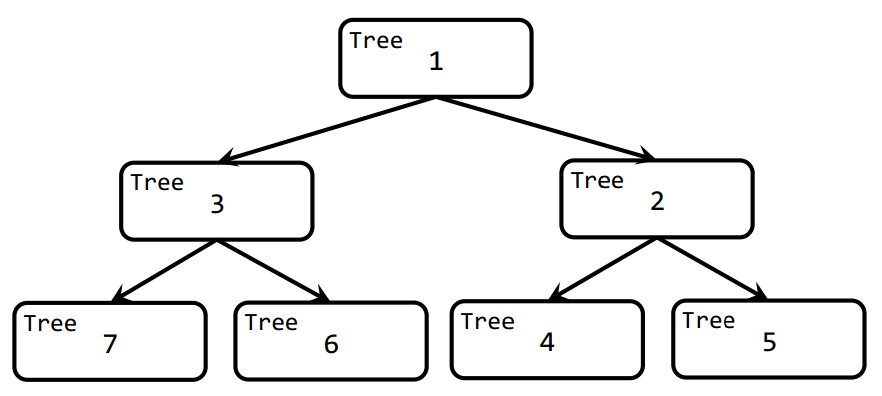
\includegraphics[width=\linewidth]{decrypted.png}
\end{minipage}

In terms of actual Python code, it should work as follows:

\begin{lstlisting}
>>> old = Tree('League of Legends accounts',
... Eert('Main account',  # swaps username and password positions
... Tree('Username: citrusdrink'),
... Tree('Password: imdiamond1'),
... Tree('Smurf account',
... Tree('Username: yummycitrusdrink'),
... Eert('Password: ishouldbeapro')))  # no children, so no swapping
>>> new = old.decrypt()
>>> old.left.left.entry  # this got swapped because of the Eert
'Password: imdiamond1'
>>> new.left.left.entry  # no longer swapped
'Username: citrusdrink'
>>> old.right.right.entry
'Password: ishouldbeapro'
>>> new.right.right.entry
'Password: ishouldbeapro'
\end{lstlisting}
\end{parts}
